%!TEX root = ../thesis.tex

\chapter{Огляд сучасних методів сегментації супутникових знімків}
\label{chap:review}

У першому розділі даної роботи ми розглянемо постановку
задачі семантичної сегментації, нейромережеві методи, які
застосовують для її розв'язку, а також специфічні проблеми,
які виникають при застосуванні цих методів до супутникових
знімків. Також мова піде про функції помилки та метрики якості
сегментації, які будуть використані у наступних розділах.

\section{Задача семантичної сегментації супутникових знімків}

Серед широко спектру задач, які пов'язані з використанням
супутникових знімків, особливе місце займає задача семантичної
сегментації. Розв'язок даної задачі дозволяє вирішувати такі прикладні задачі,
як, наприклад, детектування вирубки лісів \cite{sat_logging}, класифікацію
сільськогосподарських полів \cite{kussul2017deep}
і відіграє визначну роль у задачах моніторингу навколишнього
середовища та сільського господарства \cite{kolotii2015comparison}.

\subsection{Постановка задачі сегментації}

Як і інші задачі навчання з учителем, задача семантичної сегментації
передбачає існування навчальної вибірки, тобто набору $X$,
який складається з зображень
$I \in \left( R^C \right)^{H \times W} = \mathcal{I}$ та міток класів
$k \in K$ для кожного пікселя кожного зображення, де $R \subset \R$ --
множина можливих значень кожного каналу пікселя,
$H, W, C$ -- висота, ширина та кількість каналів зображення,
$K = \overline{1, M}$ -- множина класів ($M \in \N$ -- кількість класів).
Зазвичай множина $R = \overline{0, \dots, 255}$, або $R = [0, 1]$.

\begin{definition}\label{def:sem_segm_task}
    Нехай ми маємо навчальну вибірку $X=(I_i, Y_i)_{i=1}^{N}$,
    де $I_i \in \mathcal{I}$, $Y_i \in K^{H \times W}$.
    Задача семантичної сегментації полягає у тому, щоб
    знайти таке відображення
    $f: \mathcal{I} \rightarrow K^{H \times W}$, що деякий функціонал помилки
    $L(f, X)$ приймає мінімальне значення.
\end{definition}

Тобто задача семантичної сегментації є задачею класифікації, але
не цілого зображення, а кожного окремого пікселя.

% \begin{figure}[ht]
%     \centering
%     \begin{subfigure}[b]{0.45\textwidth}
%         \centering
%         \includegraphics[scale=0.5]{../assets/satellite.png}
%         \caption{Вхідне зображення}
%     \end{subfigure}%
%     \begin{subfigure}[b]{0.45\textwidth}
%         \centering
%         \includegraphics[scale=0.5]{../assets/mask.png}
%         \caption{Результат сегментації}
%     \end{subfigure}

%     \caption{Приклад семантичної сегментації}
%     \label{fig:segm_example}
% \end{figure}

\subsection{Функції помилки}

Важливим питанням є вибір функціоналу помилки, які може суттєво вплинути
на результат. Абсолютна більшість використовуваних на практиці
функцій помилок мають наступну форму: розраховується
певна функція помилки $l(f, p, k)$ для кожного окремого
пікселя $p \in I$, після чого застосовується певна операція редукції
по усім пікселям та зображенням. Одним з найчастіших
виборів операції редукції є звичайне середнє, і у цьому випадку
загальний функціонал помилки виглядає наступним чином:

\begin{equation} \label{eq:loss_reduction}
    L(f, X) = \frac{1}{N}
    \sum\limits_{n=1}^{N}
    \frac{1}{H \cdot W}
    \sum\limits_{(p, k) \in (I_n, Y_n)} l(f, p, k)
\end{equation}

Однією з найбільш використовуваних функцій помилки у задачах
класифікації та сегментації є крос-ентропія.

\begin{definition}[Cross-Entropy]\label{def:ce_loss}
    Нехай $p \in I$ -- піксель зображення, $k \in K$ -- правильний клас,
    $f_i(p)$ -- передбачувана ймовірність належності класу $i \in K$ для пікселя $p$, тоді крос-ентропія
    обчислюється наступним чином:
    $$ \ce(f, p, k) = - \sum\limits_{i=1}^{|K|} \ind\{i = k\} \ln f_i(p) = - \ln f_k(p) $$
\end{definition}

Інтуїтивний сенс функції крос-ентропії наступний: найменшого значення дана функція набуває тоді,
коли розподіли правильних класів та передбачуваних однакові. Тобто
дана функція є певною мірою різниці цих розподілів. Але у реальних
застосуваннях, а особливо при сегментації супутникових знімків,
дуже часто розподіл класів далекий від рівномірного, тобто
присутня незбалансованість класів. У таких випадках застосування
класичної крос-ентропії може призвести \cite{losses} до того, що
якість класифікації міноритарних класів буде низькою, бо
значення помилки буде не великим. Для того, щоб врахувати цю обставину
застосовують модифікацію, яка має назву зважена крос-ентропія.

\begin{definition}[Weighted Cross-Entropy]\label{def:wce_loss}
    Нехай $p \in I$ -- піксель зображення, $k \in K$ -- правильний клас,
    $f_i(p)$ -- передбачувана ймовірність належності класу $i \in K$ для пікселя $p$,
    $\omega_i \in (0, 1]$ -- вага класу $i \in K$.
    Тоді зважена крос-ентропія обчислюється наступним чином:
    $$ \wce(f, p, k) = - \sum\limits_{i=1}^{|K|} \omega_i \ln f_i(p) \ind\{i = k\} =
        -\omega_k \ln f_k(p) $$
\end{definition}

Тобто ми для кожного з класів задаємо ваги, тобто міру того, наскільки нам важливо
врахувати помилку у класифікації кожного пікселя цього класу. У більшості випадків,
ваги задаються $1 - \frac{N_k}{N}$, де $N_k$ - кількість пікселів класу $k$
у вибірці, $N$ - загальна кількість пікселів.

Іншою розповсюдженою функцією помилки для задач семантичної сегментації,
яка застосовна \cite{losses} при сильно незбалансованих класах є Focal Loss.

\begin{definition}[Focal Loss]\label{def:focal_loss}
    Нехай $p \in I$ -- піксель зображення, $k \in K$ -- правильний клас,
    $f_i(p)$ -- передбачувана ймовірність належності класу $i \in K$ для пікселя $p$,
    $\gamma \in (0, 1)$ -- параметр, $\omega_i \in (0, 1]$ -- вага класу $i \in K$.
    Тоді зважена Focal Loss обчислюється наступним чином:
    $$ \fl(f, p, k) = - \sum\limits_{i=1}^{|K|} \omega_i (1 - f_i(p))^\gamma \ln f_i(p) \ind\{i = k\} =
        - \omega_k (1 - f_k(p))^\gamma \ln f_k(p) $$
\end{definition}

Як можна побачити \cite{losses}, даний вигляд функції помилки дозволяє
сфокусуватися на складних прикладах та зменшити
вагу помилок тих прикладів, які вже правильно класифікуються,
але ймовірність яких все ще не рівна $1$.

Звичайно, що це далеко не повний перелік усіх можливих варіацій
функціоналу помилки, проте це найпопулярніші функції, які
широко застосовуються при розв'язанні задач семантичної
сегментації у тому числі супутникових знімків.

\subsection{Метрики якості}

Окрім визначення функціоналів помилки, для доцільно згадати й
про ті засоби, які дозволяють оцінити наскільки якісна побудована
модель семантичної сегментації.
Для надання формальних та точних оцінок, які дозволять порівнювати різні моделі
з різними функціями помилки, використовуються метрики.


\begin{definition}[IoU]\label{def:iou}

\end{definition}


\begin{definition}[Accuracy] \label{def:accuracy}

\end{definition}

\begin{definition}[User Accuracy] \label{def:user_accuracy}

\end{definition}

\begin{definition}[Producer Accuracy] \label{def:prod_accuracy}

\end{definition}

\section{Архітектура UNet}


\section{Проблеми, що виникають при застосуванні нейромережевих підходів}

Попри використання сучасних нейромережевих
архітектур, при розв'язку задач
семантичної сегментації супутникових знімків
виникають істотні проблеми, які не дозволяють
досягти максимальної якості. Ці перепони
є наслідком самої структури задачі, а саме того, що
семантична сегментація у постановці \ref{def:sem_segm_task}
є задачею навчання з учителем, тобто вимагає розміченого
набору даних, де кожному супутниковому знімку буде
відповідати відповідна ground-truth маска сегментації.

Тож першою істотною проблемою є те, що створення
навчальних вибірок, а саме: розмітка супутникових знімків,
вимагає значної кількості людських ресурсів. Причому кінцева
якість сегментації безпосередньо залежить від
розміру тренувального набору. Тобто потреба у
покращені значень метрик вимагає, серед усього іншого,
істотного збільшення навчальних прикладів,
а отже й створених людьми ground-truth масок.
Крім того, у випадку створення масок для супутникових знімків,
не завжди людина може правильно класифікувати усі об'єкти ґрунтуючись
тільки на зображенні, що може бути пов'язано з порою року,
розміром об'єкту, роздільною здатністю знімка, схожістю різних класів, тощо.

Друга істотна проблема пов'язана з дуже сильною
незбалансованістю класів, особливо у задачах класифікації
сільськогосподарських культур. Як доказ цього, можна
навести статистику (рис. \ref{fig:pixels_per_class}) ground truth
маски по кількості пікселів по кожному з
типів полів та кількості зображень, отриманих після
поділу композиту на частини по $256 \times 256$ пікселів
на яких представлений даний клас для Київської області.
Вищезгаданий поділ обумовлений тим, що нейромережеві моделі не
можуть ефективно працювати з дуже великими зображеннями,
тож ми вимушені різати їх на частини.

% \begin{figure}[ht!]
%     \centering
%     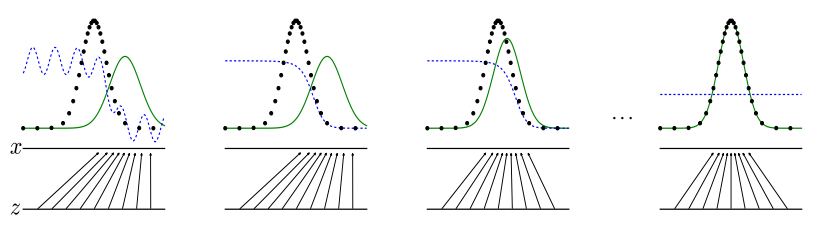
\includegraphics[height=4.5cm]{../assets/gan_distribution.png}
%     \caption{Статистики для різних класів сільськогосподарських культур}
%     \label{fig:pixels_per_class}
% \end{figure}

І попри застосування
функцій помилок, які можуть враховувати дисбаланс у
класах, досягнути бажаних значень метрик, що описують точність
моделей не вдається, що ми побачимо у подальших розділах цієї роботи.
Особливо незадовільні результати виникають саме для класів,
які мають маленьку кількість прикладів у навчальній вибірці.
А доповнити навчальну вибірку достатньою кількістю
прикладів для певних класів може бути взагалі неможливо,
через особливості сільського господарства у досліджуваному регіоні
або самої сільськогосподарської культури. Останній факт як раз
і є специфічним саме для аналізу супутникових знімків і
виділяє їх серед усіх інших сфер,
де розв'язується задача семантичної сегментації.

\chapconclude{\ref{chap:review}}


